

\tikzset{every picture/.style={line width=0.75pt}} %set default line width to 0.75pt        

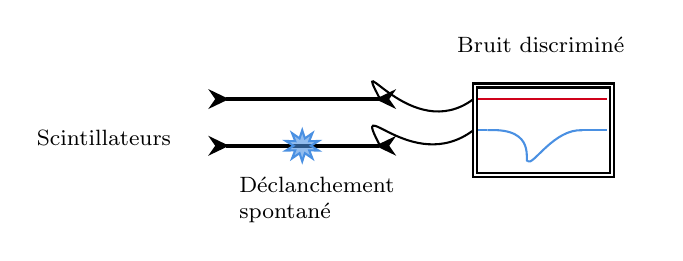
\begin{tikzpicture}[x=0.75pt,y=0.75pt,yscale=-1,xscale=1,scale=0.75]
%uncomment if require: \path (0,300); %set diagram left start at 0, and has height of 300

%Straight Lines [id:da4185804886467176] 
\draw [line width=1.5]    (201,140) -- (299,140) ;
\draw [shift={(297,140)}, rotate = 0] [fill={rgb, 255:red, 0; green, 0; blue, 0 }  ][line width=0.08]  [draw opacity=0] (13.4,-6.43) -- (0,0) -- (13.4,6.44) -- (8.9,0) -- cycle    ;
\draw [shift={(203,140)}, rotate = 180] [fill={rgb, 255:red, 0; green, 0; blue, 0 }  ][line width=0.08]  [draw opacity=0] (13.4,-6.43) -- (0,0) -- (13.4,6.44) -- (8.9,0) -- cycle    ;
%Straight Lines [id:da9391537151646601] 
\draw [line width=1.5]    (201,170) -- (299,170) ;
\draw [shift={(297,170)}, rotate = 0] [fill={rgb, 255:red, 0; green, 0; blue, 0 }  ][line width=0.08]  [draw opacity=0] (13.4,-6.43) -- (0,0) -- (13.4,6.44) -- (8.9,0) -- cycle    ;
\draw [shift={(203,170)}, rotate = 180] [fill={rgb, 255:red, 0; green, 0; blue, 0 }  ][line width=0.08]  [draw opacity=0] (13.4,-6.43) -- (0,0) -- (13.4,6.44) -- (8.9,0) -- cycle    ;
%Curve Lines [id:da4536379724430706] 
\draw    (300,140) .. controls (280.6,103) and (320,170) .. (360,140) ;
%Curve Lines [id:da13268146592186614] 
\draw    (300,170) .. controls (280.6,133) and (320,190) .. (360,160) ;
%Shape: Frame [id:dp9613596963708205] 
\draw   (360,130) -- (450,130) -- (450,190) -- (360,190) -- cycle(447.45,132.55) -- (362.55,132.55) -- (362.55,187.45) -- (447.45,187.45) -- cycle ;
%Curve Lines [id:da3104142464308661] 
\draw [color={rgb, 255:red, 74; green, 144; blue, 226 }  ,draw opacity=1 ]   (369,160) .. controls (401.8,158.2) and (392,181.4) .. (395,180) ;
%Curve Lines [id:da872976594609449] 
\draw [color={rgb, 255:red, 74; green, 144; blue, 226 }  ,draw opacity=1 ]   (430,160) .. controls (411.8,159) and (398.2,183) .. (395,180) ;
%Straight Lines [id:da5915676390224577] 
\draw [color={rgb, 255:red, 74; green, 144; blue, 226 }  ,draw opacity=1 ]   (430,160) -- (446,160) ;
%Straight Lines [id:da3011282706229732] 
\draw [color={rgb, 255:red, 208; green, 2; blue, 27 }  ,draw opacity=1 ]   (363,140) -- (446,140) ;
%Straight Lines [id:da349478425023805] 
\draw [color={rgb, 255:red, 74; green, 144; blue, 226 }  ,draw opacity=1 ]   (363,160) -- (369,160) ;
%Shape: Star [id:dp45656470082197853] 
\draw  [color={rgb, 255:red, 74; green, 144; blue, 226 }  ,draw opacity=1 ][fill={rgb, 255:red, 74; green, 144; blue, 226 }  ,fill opacity=0.6 ] (250,160) -- (251.71,165.24) -- (256.52,161.91) -- (254.48,167.06) -- (260.54,166.91) -- (255.54,170) -- (260.54,173.09) -- (254.48,172.94) -- (256.52,178.09) -- (251.71,174.76) -- (250,180) -- (248.29,174.76) -- (243.48,178.09) -- (245.52,172.94) -- (239.46,173.09) -- (244.46,170) -- (239.46,166.91) -- (245.52,167.06) -- (243.48,161.91) -- (248.29,165.24) -- cycle ;

% Text Node
\draw (140,165) node   [align=left] {\begin{minipage}[lt]{68pt}\setlength\topsep{0pt}
\footnotesize{Scintillateurs}
\end{minipage}};
% Text Node
\draw (410,105) node   [align=left] {\begin{minipage}[lt]{68pt}\setlength\topsep{0pt}
\footnotesize{Bruit discriminé}
\end{minipage}};
% Text Node
\draw (270,205) node   [align=left] {\begin{minipage}[lt]{68pt}\setlength\topsep{0pt}
\footnotesize{Déclanchement spontané}
\end{minipage}};


\end{tikzpicture}
